\documentclass[a4paper,12pt]{report}

\usepackage{alltt, fancyvrb, url}
\usepackage{graphicx}
\usepackage[utf8]{inputenc}
\usepackage{float}
\usepackage{xcolor}
\usepackage{hyperref}
\usepackage{ifluatex}
\usepackage{tabularx}
\usepackage{array}
\ifluatex
  \usepackage{pdftexcmds}
  \makeatletter
  \let\pdfstrcmp\pdf@strcmp
  \let\pdffilemoddate\pdf@filemoddate
  \makeatother
\fi
\usepackage{svg}

\usepackage[italian]{babel}
\usepackage{booktabs}

\usepackage[italian]{cleveref}
\usepackage{siunitx}

\title{Progetto di Reti\\ \textbf{Simulazione del protocollo Go-Back-N con socket UDP}}
\author{Justin Carideo\\ Matricola: 0001115610}
\date{\today}

\begin{document}

\maketitle

\newpage

\tableofcontents

\chapter{Introduzione}
Il protocollo Go-Back-N ARQ è un protocollo di comunicazione che lavora a livello del data link e permette 
la trasmissione di pacchetti dati in modo affidabile per mezzo di una 
implementazione particolare della tecnica della finestra scorrevole. 

\section{Analisi del protocollo}
Nel protocollo Go-Back-N abbiamo due entità \textit{mittente} e \textit{ricevente}
che comunicano scambiandosi pacchetti tra loro. In tutto ciò bisogna tenere
conto di:
\begin{itemize}
  \item \textit{numerazione dei pacchetti}: la numerazione sequenziale permette l'identificazione e il riordino
  \item \textit{timer di ritrasmissione}: se non viene trasmesso il pacchetto giusto ci dovrà essere un timer che ritrasmetterà dall'ultimo arrivato
  \item \textit{finestra di trasmissione del mittente}: il mittente dovrà mandare più di un pacchetto per mezzo di una finestra di lunghezza predefinita.
\end{itemize}
Ai fini pratici analizzeremo anche quando la dimensione della finestra di trasmissione è 1,
portando l'implementazione del Go-Back-N a simulare il comportamento del protocollo Stop-and-Wait.

\section{Obiettivi}
L'obiettivo è quello di implementare il protocollo tramite l'uso
di socket UDP, quindi la connessione sarà più veloce ma meno sicura rispetto
a TCP. In particolare, il tipo di protocollo è \textit{connectionless},
quindi non stabilisce una connessione tra mittente e destinatario, ma invia i pacchetti
senza alcun tipo di garanzia su ordine e integrità.
\newline
Gli obiettivi specifici dell’implementazione includono:
\begin{itemize}
  \item Ci siano due entità \textbf{server} e \textbf{client} che comunicano tra loro
  \item Fare in modo che i pacchetti siano numerati
  \item Gestire la finestra di trasmissione
  \item Implementare una funzione di timeout che permetta la ritrasmissione dei pacchetti persi
  \item Simulare la perdita di pacchetti
\end{itemize}

\chapter{Progettazione}

\section{Discussione sull'implementazione}
Per l'implementazione ho voluto dividere il lavoro tra \texttt{client} e server,
dove sono rispettivamente mittente e destinatario. Il client viene diviso in tre thread,
che hanno i seguenti ruoli:
\begin{itemize}
  \item Spedire i pacchetti in maniera sequenziale (\texttt{main})
  \item Ricevere gli ACK da parte del server (\texttt{receive\_ack})
  \item Gestire il timeout e la ritrasmissione (\texttt{handle\_timeout})
\end{itemize}
Il timer viene trattato come una risorsa condivisa tra i thread, e viene avviato, arrestato o resettato a seconda dell'invio o ricezione di pacchetti.\\
La finestra di trasmissione è definita tramite una costante che stabilisce quanti pacchetti possono essere inviati senza attendere ACK.
Per simulare la perdita dei pacchetti si è utilizzata una costante
\texttt{LOSS\_PROBABILITY}, che in combinazione con \texttt{random}
permette a \texttt{send\_pack} di non spedire in modo casuale alcuni pacchetti.\\

\section{Diagramma di flusso}
Per non mancare di generalità di seguito viene riportato il diagramma di flusso:
\begin{figure}
  \centering
  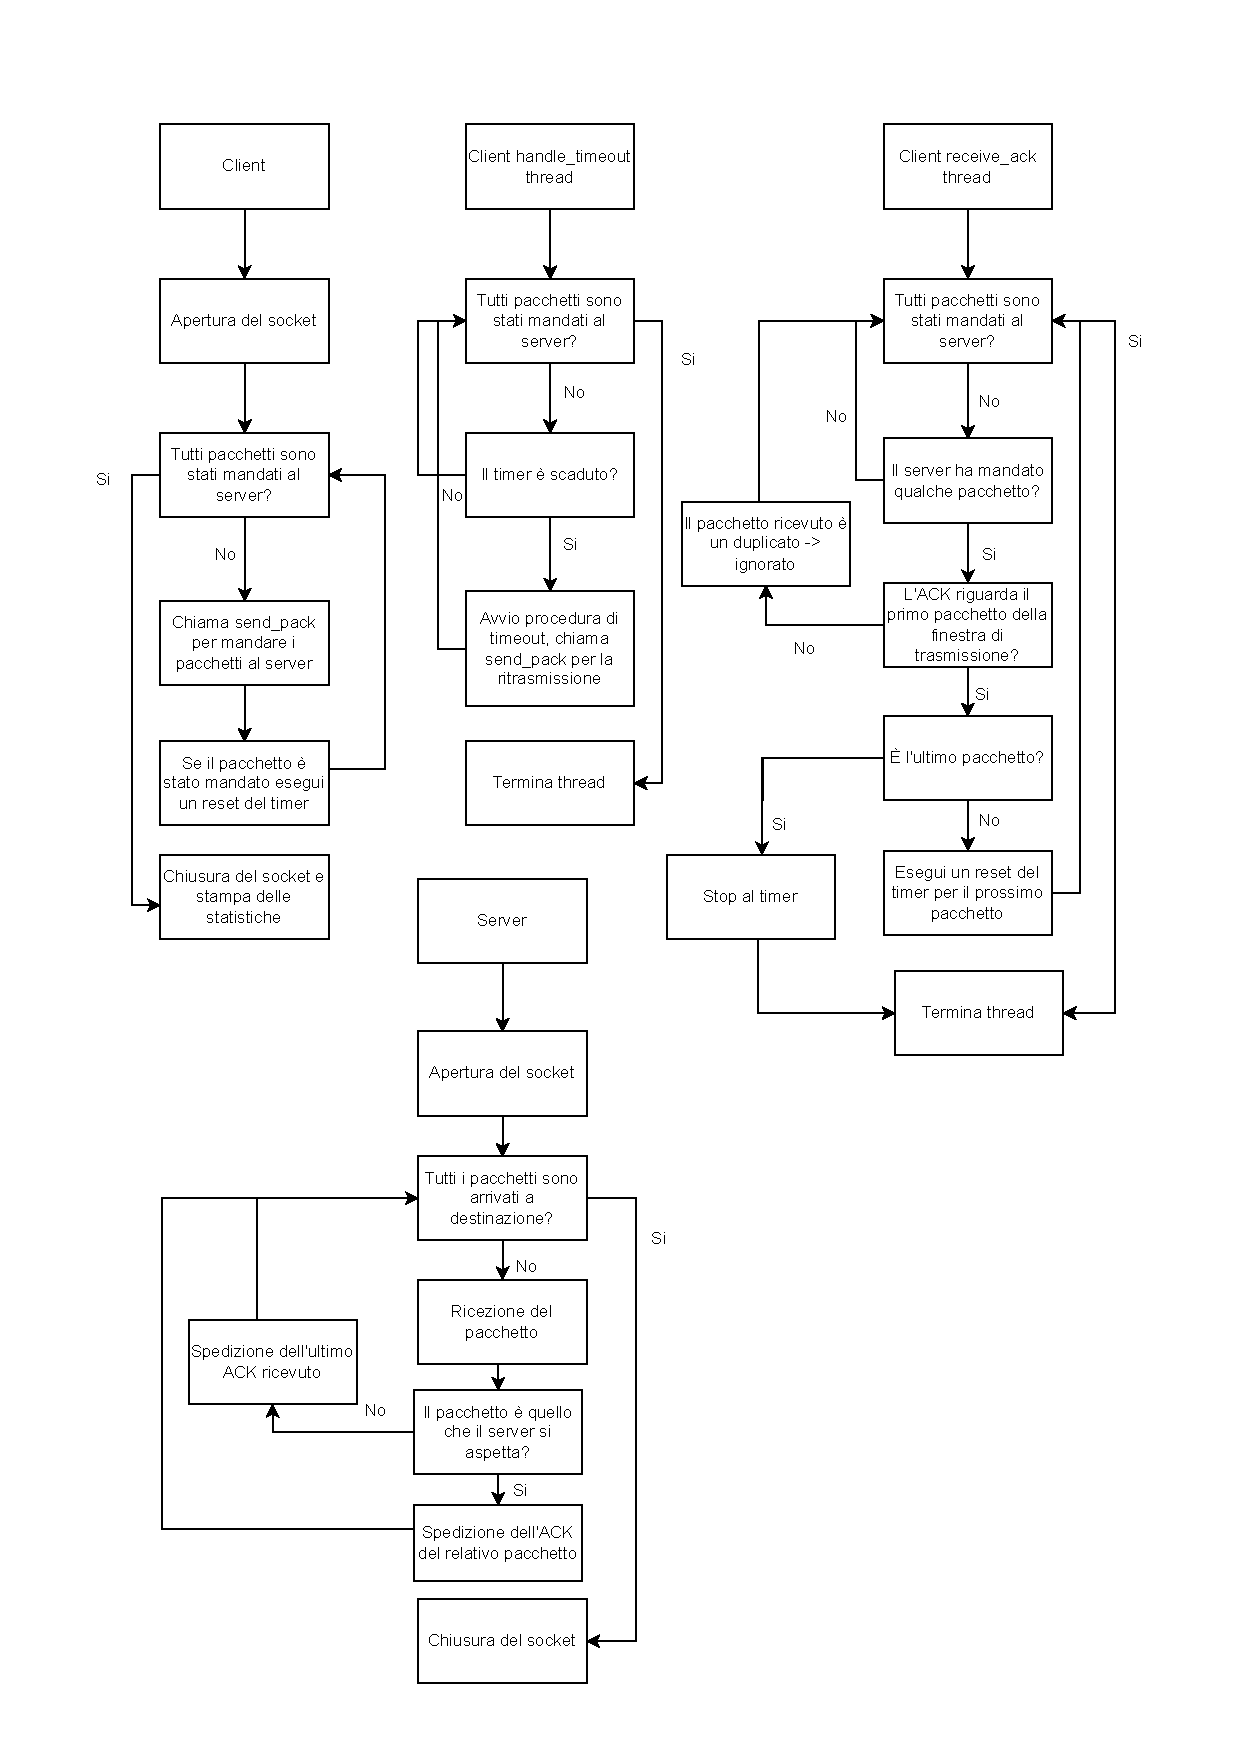
\includegraphics[width=1\textwidth]{img/GoBackN.pdf}
  \caption{Diagramma di flusso}
  \label{fig:client}
\end{figure}


\chapter{Conclusione}
Alcune particolarità le possiamo trovare nel file di log.
Se per esempio la dimensione della finestra di trasmissione è 1
si osserva che il controllo di flusso diventa quello di
uno Stop-And-Wait, dove ad ogni pacchetto spedito aspettiamo il suo 
corrispettivo ACK prima di spedirne un altro.\\
Un altro dettaglio sottile riguarda la trasmissione del primo pacchetto.
Se il primo non viene spedito e il thread di ricevimento dell'ACK prova
a chiedere di quel pacchetto, succede che viene lanciata un'eccezione
\textit{WinError 10022}, che rappresenta il fatto che il server non abbia mandato nulla.
Questo tipo di errore evidenzia l’inaffidabilità della 
comunicazione basata su UDP, poiché non viene garantita 
alcuna connessione o conferma di ricezione tra le due entità, al contrario del TCP che invece
esegue un \textit{Three-Ways-Handshake} per garantire connessione tra le entità.

\end{document}